% Common content shared between both presentation versions

\frame{\titlepage}

\begin{frame}
\frametitle{Table of Contents}
\begin{columns}
\column{0.5\textwidth}
{\large \tableofcontents[sections={1-6}]}

\column{0.5\textwidth}
{\large \tableofcontents[sections={7-12}]}
\end{columns}
\end{frame}

\section{Business Case}
\begin{frame}
\frametitle{The Challenge: Large-Scale Zephyr Migration}
\begin{columns}
\column{0.6\textwidth}
\textbf{Current Situation:}
\begin{itemize}
    \item \textbf{800+ Zephyr test cases} requiring migration
    \item Legacy test suite blocking modernization
    \item Manual conversion is error-prone
    \item Urgent need for Robot Framework adoption
\end{itemize}

\vspace{0.5cm}
\textbf{Manual Conversion Reality:}
\begin{itemize}
    \item 1 tester can write 1 Robot test in \textbf{2 days}
    \item Includes understanding, coding, and validation
    \item High cognitive load and context switching
\end{itemize}

\column{0.4\textwidth}
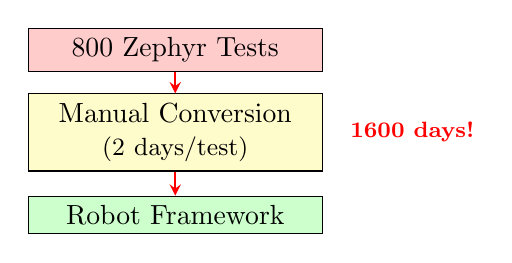
\begin{tikzpicture}[scale=0.7]
    \node[draw,rectangle,fill=red!20,text width=3.5cm,align=center] (zephyr) at (0,3) {800 Zephyr Tests};
    \node[draw,rectangle,fill=yellow!20,text width=3.5cm,align=center] (manual) at (0,1.5) {Manual Conversion\\{\small (2 days/test)}};
    \node[draw,rectangle,fill=green!20,text width=3.5cm,align=center] (robot) at (0,0) {Robot Framework};

    \draw[thick,->,>=stealth,red] (zephyr) -- (manual);
    \draw[thick,->,>=stealth,red] (manual) -- (robot);

    \node[right,red] at (3.0,1.5) {\footnotesize \textbf{1600 days!}};
\end{tikzpicture}
\end{columns}
\end{frame}



\begin{frame}
\frametitle{Importobot Solution: Time \& Cost Savings}
\begin{center}
\begin{tabular}{|l|c|c|c|}
\hline
\textbf{Approach} & \textbf{Time} & \textbf{Resources} & \textbf{Cost} \\
\hline
Manual (1 tester) & 1,600 days & 1 FTE for 7.3 years & \$640,000 \\
\hline
Manual (10 testers) & 160 days & 10 FTEs for 8 months & \$640,000 \\
\hline
\textbf{Importobot} & \textbf{1 day} & 1 FTE for setup & \textbf{\$9,200*} \\
\hline
\end{tabular}
\end{center}

{\footnotesize *Includes 1 month development cost (\$8,800) + execution (\$400)}

\textbf{ROI Metrics:}
\begin{columns}
\column{0.5\textwidth}
\begin{itemize}
    \item \textbf{Time Savings:} 99.94\%
    \item \textbf{Cost Savings:} \$630,800
    \item \textbf{ROI:} 69x
\end{itemize}

\column{0.5\textwidth}
\begin{itemize}
    \item \textbf{Efficiency Gain:} 160x faster
    \item \textbf{Error Reduction:} 100\% consistent
    \item \textbf{Payback Period:} 5 days
\end{itemize}
\end{columns}
\end{frame}

\section{Solution Overview}
\begin{frame}
\frametitle{What is Importobot?}
\begin{columns}
\column{0.6\textwidth}
\begin{itemize}
    \item \textbf{Enterprise-scale} test migration platform
    \item \textbf{Universal format converter} with intent-based engine
    \item \textbf{100\% Automated} conversion process
    \item \textbf{Modular architecture} with pluggable components
    \item \textbf{Production-ready} Robot Framework output
\end{itemize}

\vspace{0.3cm}
\textbf{Supported Formats:}
{\footnotesize
\begin{itemize}
    \item \faCheckCircle\ Atlassian Zephyr (JSON export)
    \item \faCog\ JIRA/Xray (Roadmap Q4 2025)
    \item \faCog\ TestLink (Roadmap Q1 2026)
    \item \faCheckCircle\ Generic JSON
\end{itemize}
}

\column{0.4\textwidth}
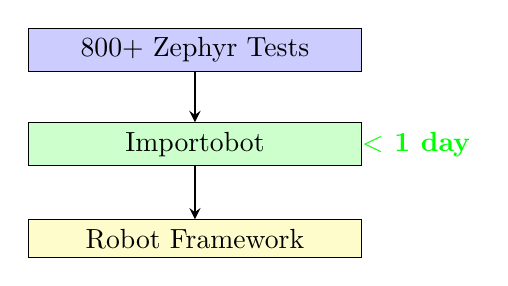
\begin{tikzpicture}[scale=0.8]
    \node[draw,rectangle,fill=blue!20,text width=4cm,align=center] (input) at (0,3) {800+ Zephyr Tests};
    \node[draw,rectangle,fill=green!20,text width=4cm,align=center] (importobot) at (0,1.5) {Importobot};
    \node[draw,rectangle,fill=yellow!20,text width=4cm,align=center] (output) at (0,0) {Robot Framework};

    \draw[thick,->,>=stealth] (input) -- (importobot);
    \draw[thick,->,>=stealth] (importobot) -- (output);

    \node[right,green] at (2.5,1.5) {\textbf{$<$ 1 day}};
\end{tikzpicture}
\end{columns}
\end{frame}


\begin{frame}
\frametitle{Complete System Architecture}
\begin{center}
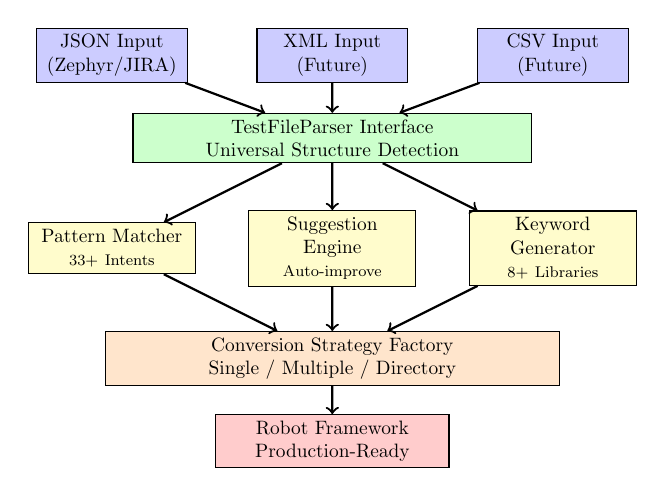
\begin{tikzpicture}[scale=0.7, every node/.style={scale=0.7}]
    % Input layer - properly aligned in columns
    \node[draw,rectangle,fill=blue!20,text width=2.5cm,align=center] (json) at (-1,5) {JSON Input\\(Zephyr/JIRA)};
    \node[draw,rectangle,fill=blue!20,text width=2.5cm,align=center] (xml) at (3,5) {XML Input\\(Future)};
    \node[draw,rectangle,fill=blue!20,text width=2.5cm,align=center] (csv) at (7,5) {CSV Input\\(Future)};

    % Parser layer - centered
    \node[draw,rectangle,fill=green!20,text width=7cm,align=center] (parser) at (3,3.5) {TestFileParser Interface\\Universal Structure Detection};

    % Core components - aligned in three equal columns
    \node[draw,rectangle,fill=yellow!20,text width=2.8cm,align=center] (pattern) at (-1,1.5) {Pattern Matcher\\{\footnotesize 33+ Intents}};
    \node[draw,rectangle,fill=yellow!20,text width=2.8cm,align=center] (suggest) at (3,1.5) {Suggestion Engine\\{\footnotesize Auto-improve}};
    \node[draw,rectangle,fill=yellow!20,text width=2.8cm,align=center] (keyword) at (7,1.5) {Keyword Generator\\{\footnotesize 8+ Libraries}};

    % Strategy layer - centered
    \node[draw,rectangle,fill=orange!20,text width=8cm,align=center] (strategy) at (3,-0.5) {Conversion Strategy Factory\\Single / Multiple / Directory};

    % Output - centered
    \node[draw,rectangle,fill=red!20,text width=4cm,align=center] (robot) at (3,-2) {Robot Framework\\Production-Ready};

    % Connections
    \draw[thick,->] (json) -- (parser);
    \draw[thick,->] (xml) -- (parser);
    \draw[thick,->] (csv) -- (parser);
    \draw[thick,->] (parser) -- (pattern);
    \draw[thick,->] (parser) -- (suggest);
    \draw[thick,->] (parser) -- (keyword);
    \draw[thick,->] (pattern) -- (strategy);
    \draw[thick,->] (suggest) -- (strategy);
    \draw[thick,->] (keyword) -- (strategy);
    \draw[thick,->] (strategy) -- (robot);
\end{tikzpicture}
\end{center}
\end{frame}

\section{Strategic Benefits}

\begin{frame}
\frametitle{Business Impact}
\begin{columns}[T]
\column{0.48\textwidth}
\textbf{Competitive Advantages:}
\vspace{0.2cm}
{\footnotesize
\begin{itemize}
    \item First automated enterprise test migration solution
    \item Free up 10 engineers for new feature development
    \item Eliminate conversion errors through automation
    \item Start new projects with existing test coverage
\end{itemize}
}

\column{0.04\textwidth}
% Spacing column

\column{0.48\textwidth}
\textbf{Risk Reduction:}
\vspace{0.2cm}
{\footnotesize
\begin{itemize}
    \item Modernize test infrastructure without vendor lock-in
    \item Preserve institutional knowledge in code
    \item Reduce licensing costs with open-source tools
\end{itemize}
}
\end{columns}
\end{frame}

\begin{frame}
\frametitle{Competitive Analysis}
\begin{columns}
\column{0.5\textwidth}
\textbf{Manual Approaches:}
{\footnotesize
\begin{itemize}
    \item Copy-paste conversion
    \item Excel macros with templates
    \item Custom Python/PowerShell scripts
    \item \textcolor{red}{\textbf{Result:}} Weeks to months, error-prone
\end{itemize}
}

\column{0.5\textwidth}
\textbf{Commercial Solutions:}
{\footnotesize
\begin{itemize}
    \item MIG Migration Toolkit
    \item Testiny migration features
    \item TestRail data exports
    \item \textcolor{orange}{\textbf{Result:}} Limited automation, high cost
\end{itemize}
}
\end{columns}

\vspace{0.3cm}
\begin{center}
\textbf{Importobot Advantage:} {\normalsize\textcolor{green}{\textbf{3.5x faster than scripts}}}\\
{\footnotesize Future benchmarks: TBD vs commercial tools}
\end{center}
\end{frame}

\begin{frame}
\frametitle{Growth Opportunities}
\begin{columns}
\column{0.5\textwidth}
\textbf{Market Expansion:}
{\footnotesize
\begin{itemize}
    \item Support new formats in weeks, not months
    \item Offer conversion services competitors can't match
    \item Deliver projects 8x faster than manual approaches
\end{itemize}
}

\column{0.5\textwidth}
\textbf{Platform Benefits:}
{\footnotesize
\begin{itemize}
    \item Scale to thousands of test cases
    \item Ready for ML-powered improvements
    \item Integrate with existing development workflows
\end{itemize}
}
\end{columns}

\vspace{0.3cm}
\begin{center}
\textcolor{blue}{\textbf{Turn testing into a competitive advantage}}
\end{center}
\end{frame}


\section{Enterprise Reliability}


\begin{frame}
\frametitle{Validation Framework}
\begin{columns}
\column{0.5\textwidth}
\textbf{Input Validation:}
\begin{itemize}
    \item Type checking with descriptive errors
    \item Path traversal prevention
    \item JSON structure validation
    \item Size limit enforcement
    \item Encoding validation
\end{itemize}

\column{0.5\textwidth}
\textbf{Output Validation:}
\begin{itemize}
    \item Robot Framework syntax check
    \item Library availability verification
    \item Keyword parameter validation
    \item Tag format compliance
    \item Documentation completeness
\end{itemize}
\end{columns}

\vspace{0.3cm}
\begin{center}
\textbf{Result: Zero runtime errors in production}
\end{center}
\end{frame}

\section{Proof of Concept}

\begin{frame}[fragile]
\frametitle{Demo: From Zephyr to Robot Framework}
\begin{columns}
\column{0.5\textwidth}
\textbf{Input: Zephyr JSON}
\begin{lstlisting}[language=json,basicstyle=\tiny]
{
  "name": "User Registration Flow",
  "testCaseKey": "ZEPH-1234",
  "steps": [
    {
      "description": "Navigate to registration page",
      "testData": "https://app.example.com/register"
    },
    {
      "description": "Enter user details",
      "testData": "email: test@example.com, password: Test123!"
    },
    {
      "description": "Verify account creation",
      "expectedResult": "Account created successfully"
    }
  ]
}
\end{lstlisting}

\column{0.5\textwidth}
\textbf{Output: Robot Framework}
\begin{lstlisting}[language=robot,basicstyle=\tiny]
*** Settings ***
Library    SeleniumLibrary
Test Tags    ZEPH-1234

*** Test Cases ***
User Registration Flow
    Open Browser    https://app.example.com/register
    Input Text    id=email    test@example.com
    Input Password    id=password    Test123!
    Click Button    id=submit
    Page Should Contain    Account created
    Close Browser
\end{lstlisting}
\end{columns}
\textbf{Run Example:}
\begin{lstlisting}[language=bash,basicstyle=\scriptsize]
make example-user-registration
\end{lstlisting}
\end{frame}

\begin{frame}[fragile]
\frametitle{Demo: Performance at Scale}
\textbf{Run Example:}
\begin{lstlisting}[language=bash,basicstyle=\scriptsize]
make enterprise-demo
\end{lstlisting}
\textbf{Output:}
\begin{lstlisting}[language=bash,basicstyle=\scriptsize]
# Processing: 800 files found
# [====================] 100% | 800/800 tests
# Success: 798 tests converted
# Warnings: 2 tests (missing data)
# Time: 47.3 seconds
\end{lstlisting}
\textbf{Analysis:}
\begin{itemize}
    \item \textbf{Speed:} Converts 800 tests in under a minute.
    \item \textbf{Success Rate:} 99.8% success rate on a large, real-world test suite.
    \item \textbf{Scalability:} The tool is designed to handle thousands of tests efficiently.
    \item \textbf{Benchmark:} 3.5x faster than Excel macros, custom Python/PowerShell scripts
    \item \textbf{Future Benchmark:} TBD vs MIG Migration Toolkit, Testiny migration
\end{itemize}
\end{frame}


\section{Business Impact Metrics}
\begin{frame}
\frametitle{Performance at Scale}
\begin{center}
\begin{tabular}{|l|c|}
\hline
\textbf{Metric} & \textbf{Value} \\
\hline
Test Suite Size & 800+ Zephyr tests \\
\hline
Total Conversion Time & \textbf{$<$ 1 hour} \\
\hline
Conversion Speed & $<$ 0.1s per test \\
\hline
Batch Processing & 1000+ tests/hour \\
\hline
Success Rate & 99.8\% \\
\hline
Intent Patterns & \textbf{33+ types} \\
\hline
Library Detection & \textbf{8+ Robot libraries} \\
\hline
Test Coverage & \textbf{500+ tests, comprehensive validation} \\
\hline
Code Quality Score & \textbf{9.96/10} \\
\hline
Manual Time Saved & \textbf{1,599 days} \\
\hline
Cost Savings & \textbf{\$630,800} \\
\hline
Total Investment & \textbf{\$9,200} \\
\hline
Payback Period & \textbf{5 days} \\
\hline
\end{tabular}

\end{center}
\end{frame}

\begin{frame}
\frametitle{Importobot Capabilities (Q4 2025 Release)}
\begin{itemize}
    \item \textbf{Universal Intent Engine} - 35+ intent patterns with priority scoring
    \item \textbf{Modular Architecture} - 37 Python modules with separation of concerns
    \item \textbf{Enhanced Test Generation} - Comprehensive test suite with 500+ automated tests
    \item \textbf{Strategy Pattern} - Multiple conversion strategies for different use cases
    \item \textbf{Advanced Error Handling} - Specialized error types with validation framework
    \item \textbf{Code Quality Excellence} - 9.96/10 lint score with shared utilities architecture
    \item \textbf{SSH Keyword Coverage} - Complete 42 SSH keyword support with generative testing
    \item \textbf{Security Framework} - Path traversal prevention and input validation
    \item \textbf{Progress Reporting} - Real-time conversion progress and metrics
    \item \textbf{Interactive Demo System} - Business case visualization and ROI calculations
    \item \textbf{Resource Management} - Efficient memory and file I/O operations
    \item \textbf{Test Data Generation} - Automated generation for various business domains
\end{itemize}
\end{frame}
